\documentclass[tikz,border=0pt]{standalone}\newif\iftext\textfalse\begin{document}
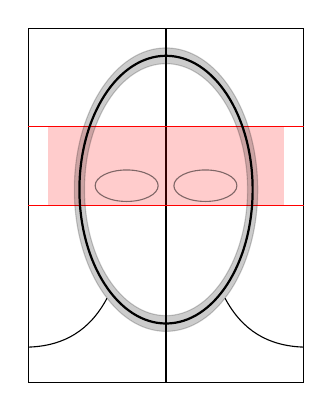
\begin{tikzpicture}[x=1mm,y=1mm,font=\sffamily\bfseries,sloped]
    % cadre
    \draw (0,0) coordinate(LL) rectangle +(35, 45) coordinate(UR);
    \draw (35/2,0) -- +(0,45);
    \iftext
    	\draw[ultra thick,latex-latex] (0,-4) -- node[fill=white]{35 mm}+(35,0);
    	\draw[ultra thick,latex-latex] (35+4,0) -- node[fill=white]{45 mm}+(0,45);
    \fi
    % zone des yeux
    \draw[red] (0,45/2) -- +(35,0);
    \draw[red] (0,45/2+10) -- +(35,0);
    \fill[red, opacity=.2]  (2.5,45/2) rectangle +(30,10);
    \draw[opacity=.5] (35/2,45/2) \foreach\i in {-1,1}{+(\i*5,2.5) ellipse(4 and 2)};
    \iftext
        \node[opacity=.7,scale=.7] at (35/2,45/2+7){zone des yeux};
    \fi
    % zone visage
    \begin{scope}[shift={(0,45/2+2)}]
        \iftext
            \draw (-7,18) -- +(30,0) (-7,-18) -- +(30,0);
            \draw[thick,latex-latex] (-5,-18) -- node[gray,fill=white,scale=.7]{36 mm}(-5,18);
            \draw (-4,16) -- +(30,0) (-4,-16) -- +(30,0);
            \draw[thick,latex-latex] (-2,-16) -- node[gray,fill=white,scale=.7]{32 mm}(-2,16);
        \fi
        \draw[thick] (35/2,0) ellipse[x radius=11,y radius=17];
        \draw[fill,even odd rule,opacity=.2] (35/2,0)
    		foreach \i in {{32/34},{36/34}}{
    			ellipse[scale=\i,x radius=11,y radius=17]};
    \end{scope}
    % epaules
    \draw (0,4.5) to[bend right] (10,10.7) [shift={(35,0)},xscale=-1](0,4.5) to[bend right] (10,10.7);
\end{tikzpicture}
\end{document}
